\documentclass[11pt,a4paper]{article}

\usepackage[margin=1in]{geometry}
\usepackage{graphicx}
\usepackage{booktabs}
\usepackage{longtable}
\usepackage{tabularx}
\usepackage{multirow}
\usepackage{amsmath}
\usepackage{amssymb}
\usepackage{siunitx}
\usepackage{hyperref}
\usepackage{xcolor}
\usepackage{caption}
\usepackage{subcaption}
\usepackage{enumitem}
\usepackage[round]{natbib}

\setlength{\emergencystretch}{2em}
% Keep floats near discussion without sacrificing readable figure/table type.
\renewcommand{\topfraction}{0.85}
\renewcommand{\bottomfraction}{0.75}
\renewcommand{\textfraction}{0.10}
\renewcommand{\floatpagefraction}{0.80}
\setcounter{topnumber}{3}
\setcounter{totalnumber}{4}
\captionsetup{font=small,skip=6pt}
\captionsetup[table]{position=top}
\setlength{\textfloatsep}{14pt plus 2pt minus 2pt}
\setlength{\floatsep}{12pt plus 2pt minus 2pt}

\hypersetup{
    colorlinks=true,
    hypertexnames=false,
    linkcolor=blue,
    citecolor=blue,
    urlcolor=blue,
    pdftitle={Profiling Sparse-Index Gradient Accumulation in Backpropagation}
}

\begin{document}

\begin{titlepage}
    \centering
    \vspace*{1.5cm}
    {\LARGE\bfseries Tie-Aware Characterization of Sparse-Index Gradient Accumulation for PyTorch CUDA Backpropagation\par}
    \vspace{2cm}
    {\large Marko Mihajlovic\par}
    \vspace{0.5cm}
    {\large Singidunum University\par}
    \vspace{0.25cm}
    {\large Belgrade, Serbia\par}
    \vspace{0.25cm}
    {\large E-mail: marko.mihajlovic.23@singimail.rs\par}
    \vspace{0.25cm}
    {\large ORCID: 0009-0006-7979-0341\par}
    \vspace{0.5cm}
    {\large 2026\par}
    \vfill
    {\itshape Journal-independent working draft\par}
\end{titlepage}
\begin{abstract}
% TODO: Write after finalizing the results narrative.
\end{abstract}

\noindent\textbf{Keywords:} sparse gradients; backpropagation; PyTorch; CUDA; embedding backward; index add; scatter add; AI model training
\section{Introduction}

Modern AI training workloads are not composed only of dense matrix multiplication, convolution, or attention kernels. Many practical models also contain sparse or irregular components whose performance is shaped by index distributions, memory access patterns, and reduction behavior. This is especially visible in recommendation and sparse-feature models, where large embedding tables are used to represent categorical identifiers and where training efficiency depends on both dense neural-network computation and memory-intensive embedding operations \citep{naumov2019dlrm,gupta2020architectural}. Recent work on large-scale embedding optimization further shows that embedding access patterns, repeated indices, and gradient processing remain important systems-level concerns in recommendation-model training \citep{liu2024embark}.

A central operation in such workloads is sparse-index gradient accumulation during backpropagation. In the forward pass, indexed operations such as embedding lookup gather rows from a parameter table. In the backward pass, gradients associated with those indexed rows must be routed back and accumulated into the corresponding parameter-gradient structure. When the same index appears multiple times in a batch, several gradient contributions target the same destination row. This creates an indexed aggregation problem rather than a purely dense tensor operation. The cost of this aggregation can depend on the number of rows, number of indices, feature dimension, index skew, duplicate-index frequency, memory layout, and the CUDA execution path selected by the framework.

From a parallel-computing perspective, these operations are instances of irregular indexed reduction: many source vectors update a smaller set of destination rows, and duplicate or skewed indices create contention, ordering, and memory-access effects. This makes stack-sensitive performance behavior a performance-portability concern for high-level GPU tensor APIs, beyond API convenience in machine-learning code.

We use PyTorch as the experimental framework \citep{paszke2019pytorch}. The compared paths are direct indexed accumulation through \texttt{index\_add} and \texttt{scatter\_add}, and gradient accumulation through \texttt{Embedding.backward}. Our workload construction makes their dense row-gradient outputs comparable; it does not assume identical API contracts or internal execution paths. The operator names identify the implementations evaluated here, rather than implying interchangeable kernel behavior.

CUDA kernel execution is asynchronous with respect to the host, making synchronization-aware timing essential \citep{nvidia2026cudaguide}. Repeated measurements, variability reporting, and reproducible experimental conditions are also central to scientific performance comparisons \citep{hoefler2015benchmarking}. We therefore separate unprofiled CUDA-event timing from profiler-based execution-path attribution and validate numerical outputs before accepting timing rows.

Prior work develops sparse GPU kernels \citep{gale2020sparse} and optimizes GPU recommendation training and embedding-gradient processing \citep{mudigere2022neo,liu2024embark}. These studies connect performance to workload structure and execution strategy. Our question concerns the high-level framework interface: how do standard PyTorch CUDA paths compare under matched sparse-index gradient accumulation workloads, and how should practical ties inform implementation choice?

This paper addresses that question through a controlled empirical study of sparse-index gradient accumulation during backpropagation-style computation. The study evaluates standard PyTorch CUDA paths rather than custom CUDA kernels. It first calibrates the benchmark protocol and validation rules, then performs a matched grid-level timing comparison, uses representative profiler runs to relate timing behavior to CUDA execution paths, and finally adds a small training-step proxy to examine whether isolated sparse-index accumulation behavior remains visible in a broader backward-style computation. The main systems contribution is a reproducible performance characterization and measurement-backed interpretation framework for workload-, scope-, and stack-dependent behavior, culminating in a tie-aware selection protocol.

The paper makes five contributions:
\begin{itemize}
\item A correctness-gated, reproducible comparison of three standard PyTorch CUDA sparse-index accumulation paths: \texttt{index\_add}, \texttt{scatter\_add}, and \texttt{Embedding.backward}.
\item Evidence of workload-, scope-, and stack-dependent behavior across the GTX1650Ti and hosted Colab T4 stacks, using matched isolated benchmarks and a backward-style proxy.
\item Profiler-backed evidence of distinct CUDA execution-path compositions, interpreted at the stack level rather than as isolated hardware causality.
\item Threshold-sensitivity and descriptive bootstrap checks, winner maps, and regret/minimax analyses that contextualize practical ties and quantify static-selection costs.
\item A measurement-backed, tie-aware selection protocol for comparing candidate paths under the target workload and execution stack.
\end{itemize}

The rest of the paper is organized as follows. Section~\ref{sec:background-related-work} reviews sparse operations in AI training, embedding-heavy workloads, indexed accumulation APIs, CUDA execution behavior, and related profiling methodology. Section~\ref{sec:methodology} describes the benchmark scope, workload design, correctness validation, timing methodology, profiling methodology, and cross-environment comparison. Section~\ref{sec:results-analysis} presents the calibrated benchmark results, matched Phase 2 timing evidence, representative Phase 3 profiler results, the Phase 4 training-step proxy, and result-level discussion. Section~\ref{sec:general-discussion} discusses significance, practical implications, limitations, generalizability, and future work. Section~\ref{sec:conclusion} concludes the paper.
\section{Background and Related Work}

% TODO: Discuss sparse operations in AI training.
% TODO: Discuss embedding gradients and recommender-style workloads.
% TODO: Discuss scatter/reduce patterns in backpropagation.
% TODO: Describe PyTorch CUDA execution paths.
% TODO: Review related benchmarking and profiling work.
% TODO: Identify the research gap.
% TODO: Add citations on embedding backward implementations and scatter/reduce CUDA behavior.
\section{Methodology}

\subsection{Study Scope}
% TODO: Define the study scope.

\subsection{Benchmarked Operations}
% TODO: Describe index_add, scatter_add, and Embedding.backward.

\subsection{Workload Design}
% TODO: Describe dimensions, distributions, indices, rows, and workload seeds.

\subsection{Correctness Validation}
% TODO: Describe numerical correctness checks.

\subsection{Timing Methodology}
% TODO: Describe timing and synchronization methodology.

\subsection{Profiling Methodology}
% TODO: Describe profiler configuration and kernel attribution.

\subsection{Cross-Environment Comparison}
% TODO: Describe matched Phase 2 and Phase 3 environment comparisons.

\subsection{Threats to Validity}
% TODO: Discuss threats to validity.

% Source artifacts:
% - ./sparse-gradient/phase2_analysis_v2/
% - ./sparse-gradient/phase3_profile_local_v2/
% - ./sparse-gradient/phase3_profile_t4_v2/
% - ./sparse-gradient/phase3_comparison_v2/
\section{Results and Analysis}

\subsection{Matched Phase 2 Benchmark Results}
% TODO: Use phase2_analysis_v2/phase2_analysis_report.md.
% TODO: % Source: ../sparse-gradient/phase2_analysis_v2/winner_counts_by_run.csv
\begin{table}[tbp]
\centering
\small
\caption{Draft: Phase 2 winner counts by environment and operation.}
\label{tab:phase2-winner-counts}
\resizebox{\linewidth}{!}{%
\begin{tabular}{llrrrrrr}
\toprule
Environment & Operation & Per-draw wins & Per-draw rate & Non-noise wins & Non-noise rate & Draws \\
\midrule
GTX1650Ti & index\_add & 123 & 0.3796 & 121 & 0.3735 & 324 \\
GTX1650Ti & scatter\_add & 0 & 0.0000 & 0 & 0.0000 & 324 \\
GTX1650Ti & embedding & 201 & 0.6204 & 193 & 0.5957 & 324 \\
GTX1650Ti & embedding\_bag & 0 & 0.0000 & 0 & 0.0000 & 324 \\
GTX1650Ti & sorted\_segment & 0 & 0.0000 & 0 & 0.0000 & 324 \\
T4 & index\_add & 21 & 0.0648 & 0 & 0.0000 & 324 \\
T4 & scatter\_add & 260 & 0.8025 & 223 & 0.6883 & 324 \\
T4 & embedding & 43 & 0.1327 & 41 & 0.1265 & 324 \\
T4 & embedding\_bag & 0 & 0.0000 & 0 & 0.0000 & 324 \\
T4 & sorted\_segment & 0 & 0.0000 & 0 & 0.0000 & 324 \\
T4\_repeat & index\_add & 7 & 0.0432 & 0 & 0.0000 & 162 \\
T4\_repeat & scatter\_add & 124 & 0.7654 & 111 & 0.6852 & 162 \\
T4\_repeat & embedding & 31 & 0.1914 & 27 & 0.1667 & 162 \\
\bottomrule
\end{tabular}
}%
\end{table}

\subsection{Representative Phase 3 Profiling Results}
% TODO: Use phase3_comparison_v2/phase3_comparison_report.md.
% TODO: % Source: ../sparse-gradient/phase3_comparison_v2/phase3_kernel_category_summary.csv
% TODO: Expand this draft import to the selected full-event rows before finalizing tables.
\begin{table}[tbp]
\centering
\small
\caption{Draft: CUDA kernel-category summary import schema.}
\label{tab:phase3-kernel-category-summary}
\begin{tabular}{llllrr}
\toprule
Environment & Case & Operation & Category & CUDA time (ms) & CUDA share \\
\midrule
GTX1650Ti & case01 & embedding & arange\_index\_setup & 0.012672 & 0.010926 \\
GTX1650Ti & case01 & embedding & embedding\_accumulate & 0.890322 & 0.767673 \\
GTX1650Ti & case01 & embedding & sort\_scan\_unique & 0.225956 & 0.194829 \\
GTX1650Ti & case01 & embedding & zero\_fill\_memset & 0.030818 & 0.026573 \\
GTX1650Ti & case01 & index\_add & index\_add\_accumulate & 0.983863 & 0.983809 \\
GTX1650Ti & case01 & index\_add & zero\_fill\_memset & 0.016192 & 0.016191 \\
GTX1650Ti & case01 & scatter\_add & scatter\_add\_accumulate & 3.141556 & 0.995024 \\
GTX1650Ti & case01 & scatter\_add & zero\_fill\_memset & 0.015711 & 0.004976 \\
\bottomrule
\end{tabular}
\end{table}
% TODO: \begin{figure}[tbp]
% TODO: \centering
% TODO: 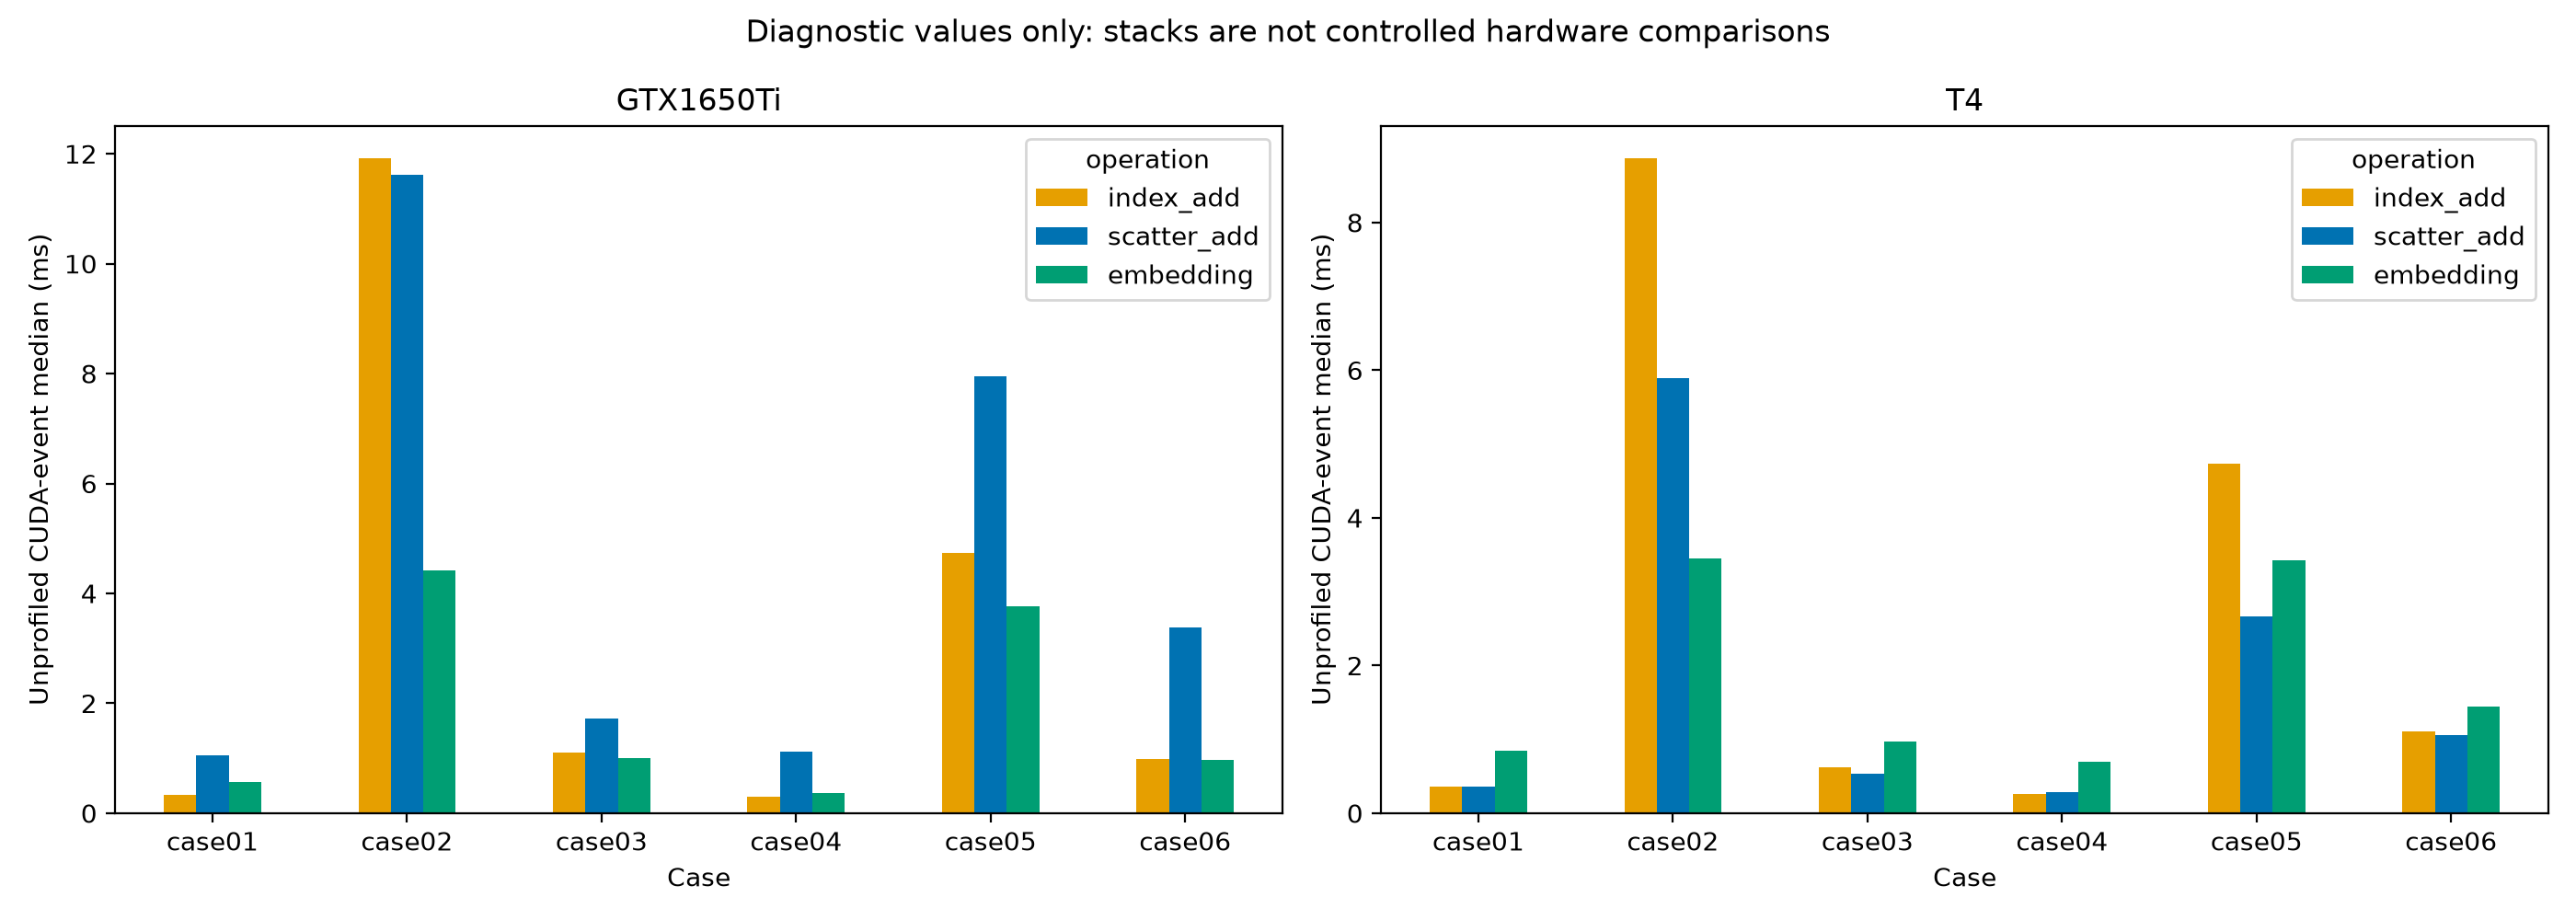
\includegraphics[width=0.80\linewidth]{figures/phase3_median_ms_by_case_operation.png}
% TODO: \caption{Draft: Phase 3 median time by case and operation.}
% TODO: \label{fig:phase3-median-ms}
% TODO: \end{figure}
% TODO: \begin{figure}[tbp]
% TODO: \centering
% TODO: 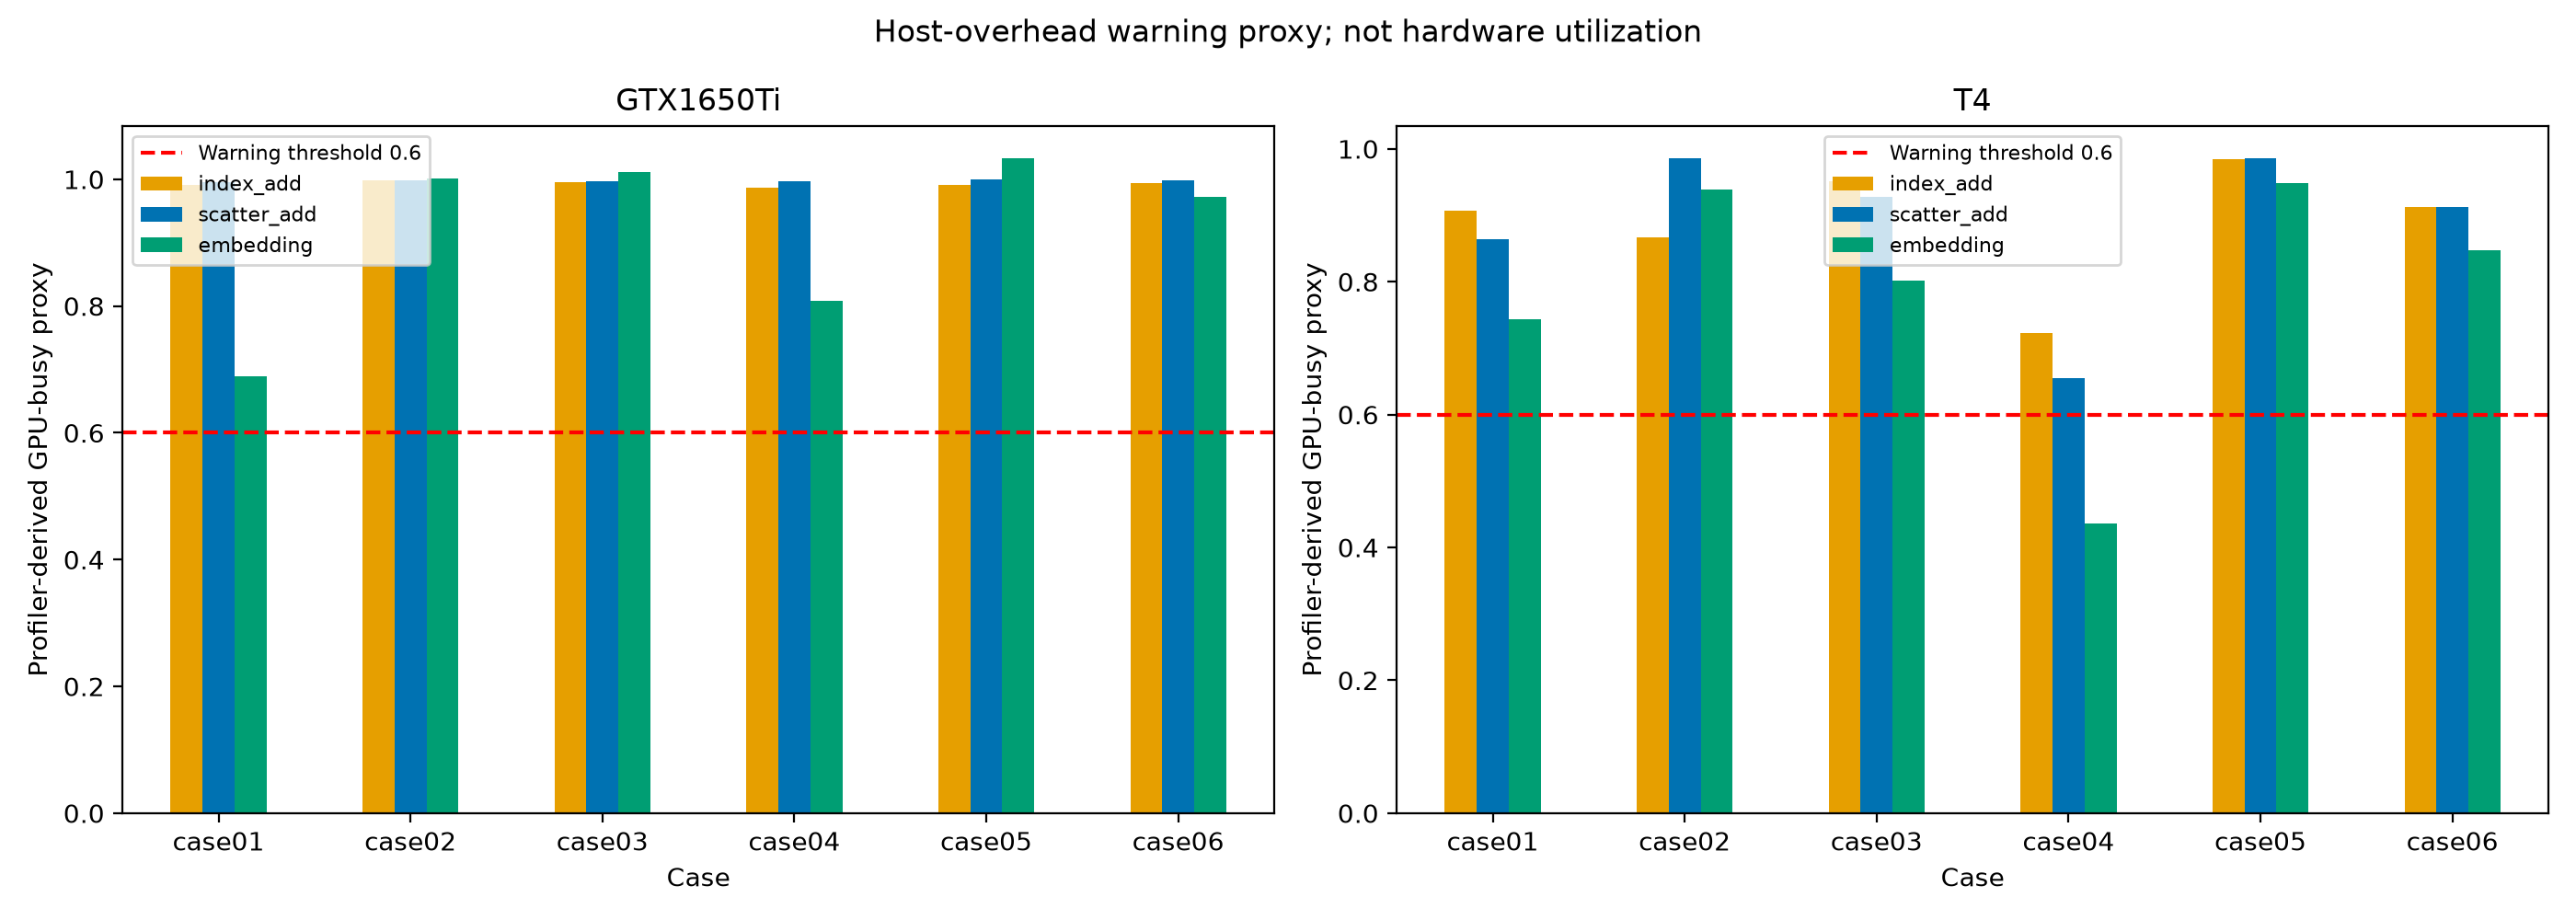
\includegraphics[width=0.80\linewidth]{figures/phase3_gpu_busy_fraction_by_case_operation.png}
% TODO: \caption{Draft: Phase 3 GPU busy fraction by case and operation.}
% TODO: \label{fig:phase3-gpu-busy}
% TODO: \end{figure}
% TODO: \begin{figure}[tbp]
% TODO: \centering
% TODO: 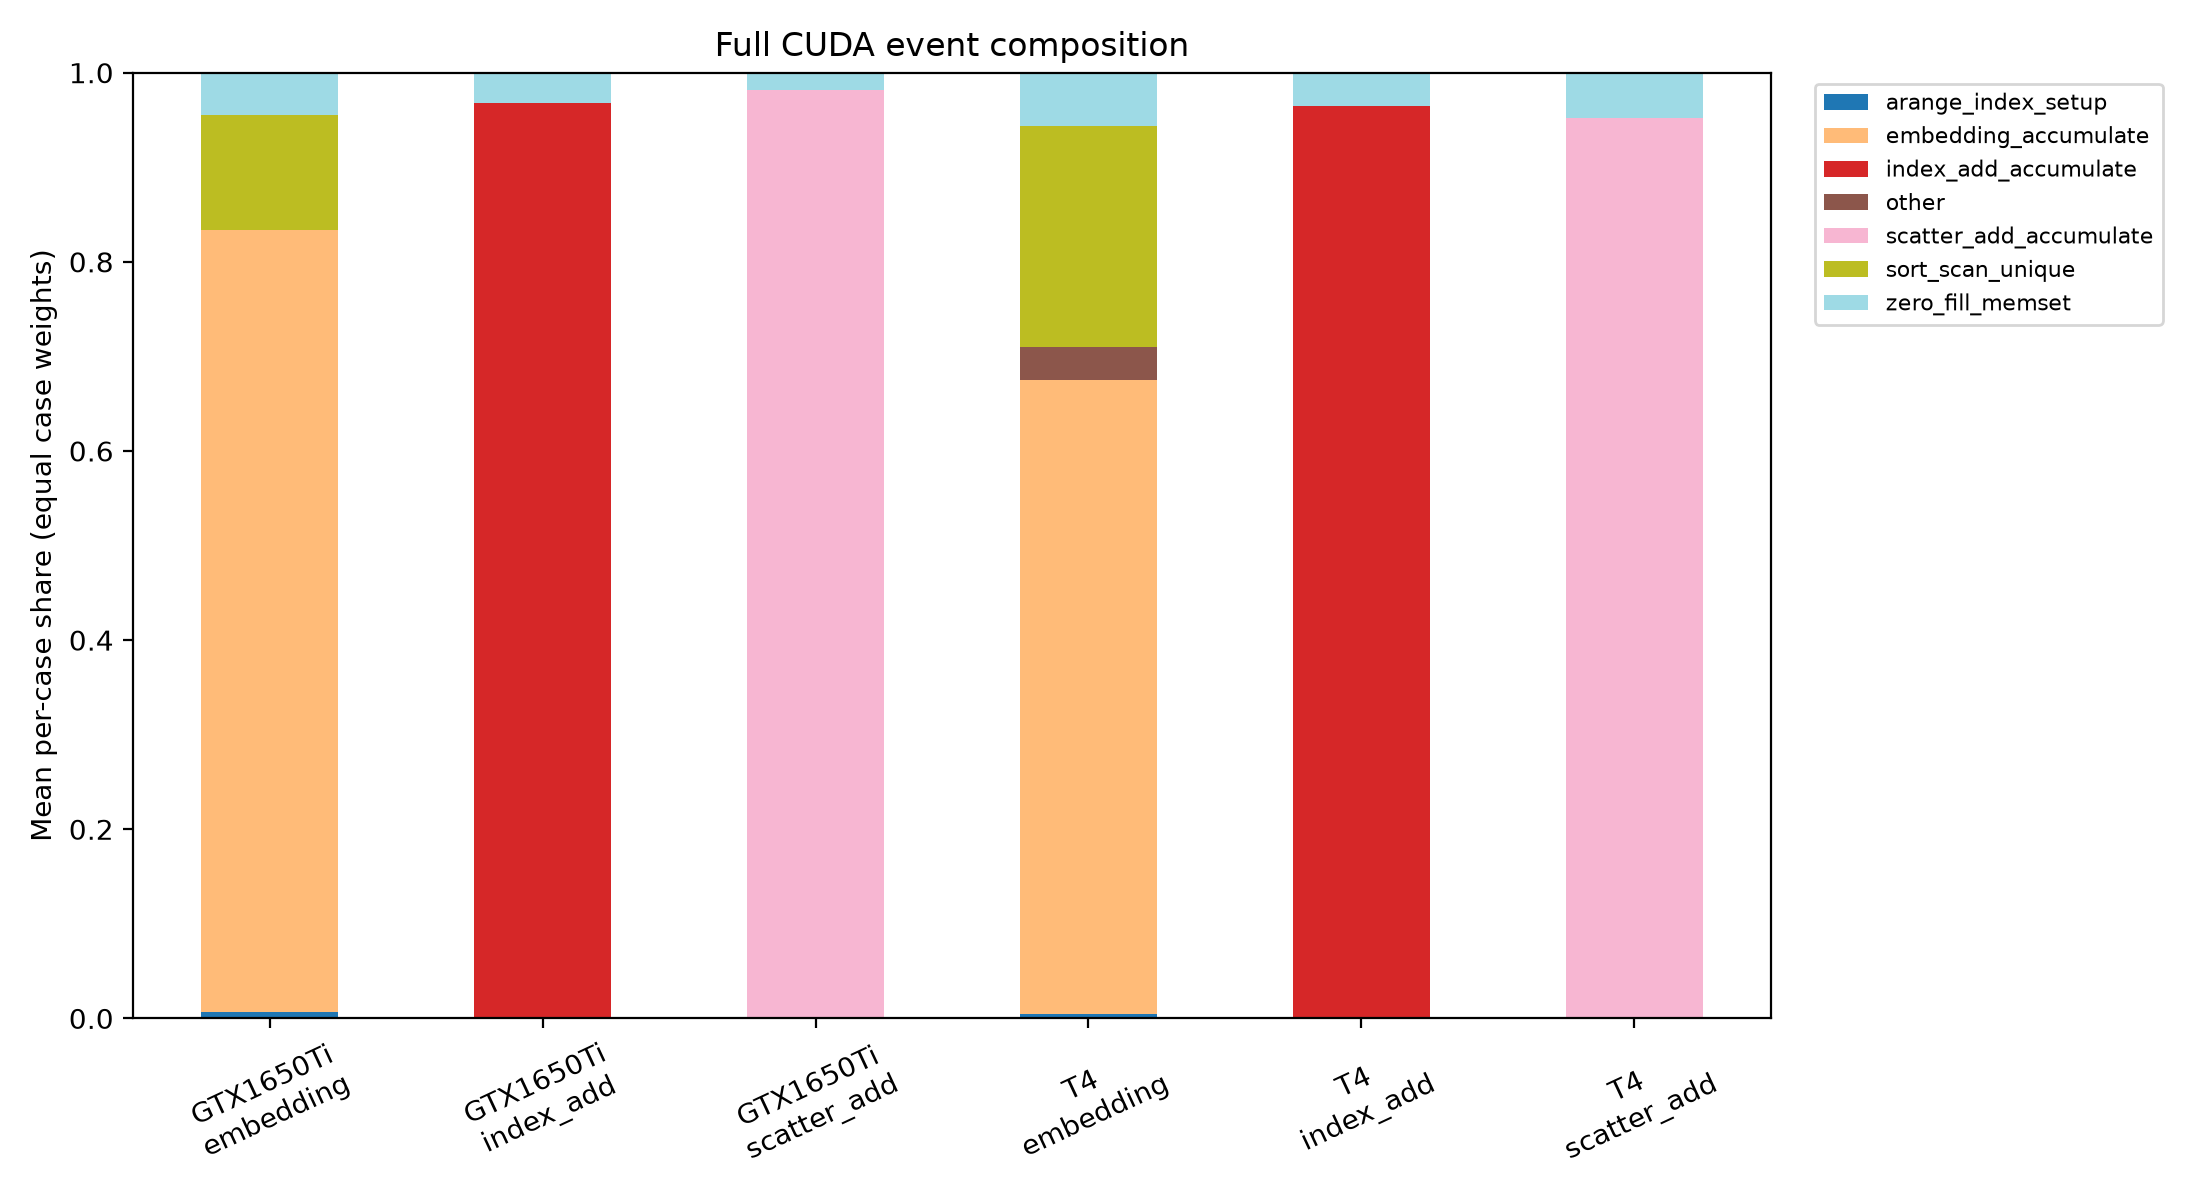
\includegraphics[width=0.80\linewidth]{figures/phase3_kernel_category_share.png}
% TODO: \caption{Draft: Phase 3 CUDA kernel-category share.}
% TODO: \label{fig:phase3-kernel-category-share}
% TODO: \end{figure}

\subsection{Case-Level Cross-Environment Comparison}
% TODO: Use phase3_comparison_v2/phase3_case_comparison.csv.
% TODO: Use phase3_comparison_v2/phase3_phase2_case_join.csv.
% TODO: % Source: ../sparse-gradient/phase3_comparison_v2/phase3_case_comparison.csv
\begin{table}[tbp]
\centering
\small
\caption{Draft: Phase 3 case-level comparison across environments.}
\label{tab:phase3-case-comparison}
\begin{tabular}{lrrrrll}
\toprule
Case & Local winner & T4 winner & Local margin & T4 margin & Relation & Pairing \\
\midrule
case01 & index\_add & scatter\_add & 1.670 & 1.022 & reversal\_near\_tie & exact \\
case02 & embedding & embedding & 2.631 & 1.706 & same\_decisive & exact \\
case03 & embedding & scatter\_add & 1.116 & 1.186 & reversal\_decisive & exact \\
case04 & index\_add & index\_add & 1.197 & 1.058 & same\_decisive & exact \\
case05 & embedding & scatter\_add & 1.257 & 1.285 & reversal\_decisive & exact \\
case06 & embedding & scatter\_add & 1.015 & 1.040 & reversal\_near\_tie & exact \\
\bottomrule
\end{tabular}
\end{table}
% TODO: % Source: ../sparse-gradient/phase3_comparison_v2/phase3_phase2_case_join.csv
\begin{table}[tbp]
\centering
\small
\caption{Draft: Matched Phase 2 and Phase 3 case winners.}
\label{tab:phase3-phase2-case-join}
\begin{tabular}{lllllll}
\toprule
Case & Phase 2 local & Phase 2 T4 & Phase 2 T4 repeat & Local agree & T4 agree & Phase 3 local/T4 \\
\midrule
case01 & index\_add & tie & tie & True & False & index\_add / scatter\_add \\
case02 & embedding & embedding & embedding & True & True & embedding / embedding \\
case03 & embedding & scatter\_add & scatter\_add & True & True & embedding / scatter\_add \\
case04 & index\_add & tie & tie & True & False & index\_add / index\_add \\
case05 & embedding & scatter\_add & scatter\_add & True & True & embedding / scatter\_add \\
case06 & tie & index\_add & tie & False & False & embedding / scatter\_add \\
\bottomrule
\end{tabular}
\end{table}
% TODO: \begin{figure}[tbp]
% TODO: \centering
% TODO: 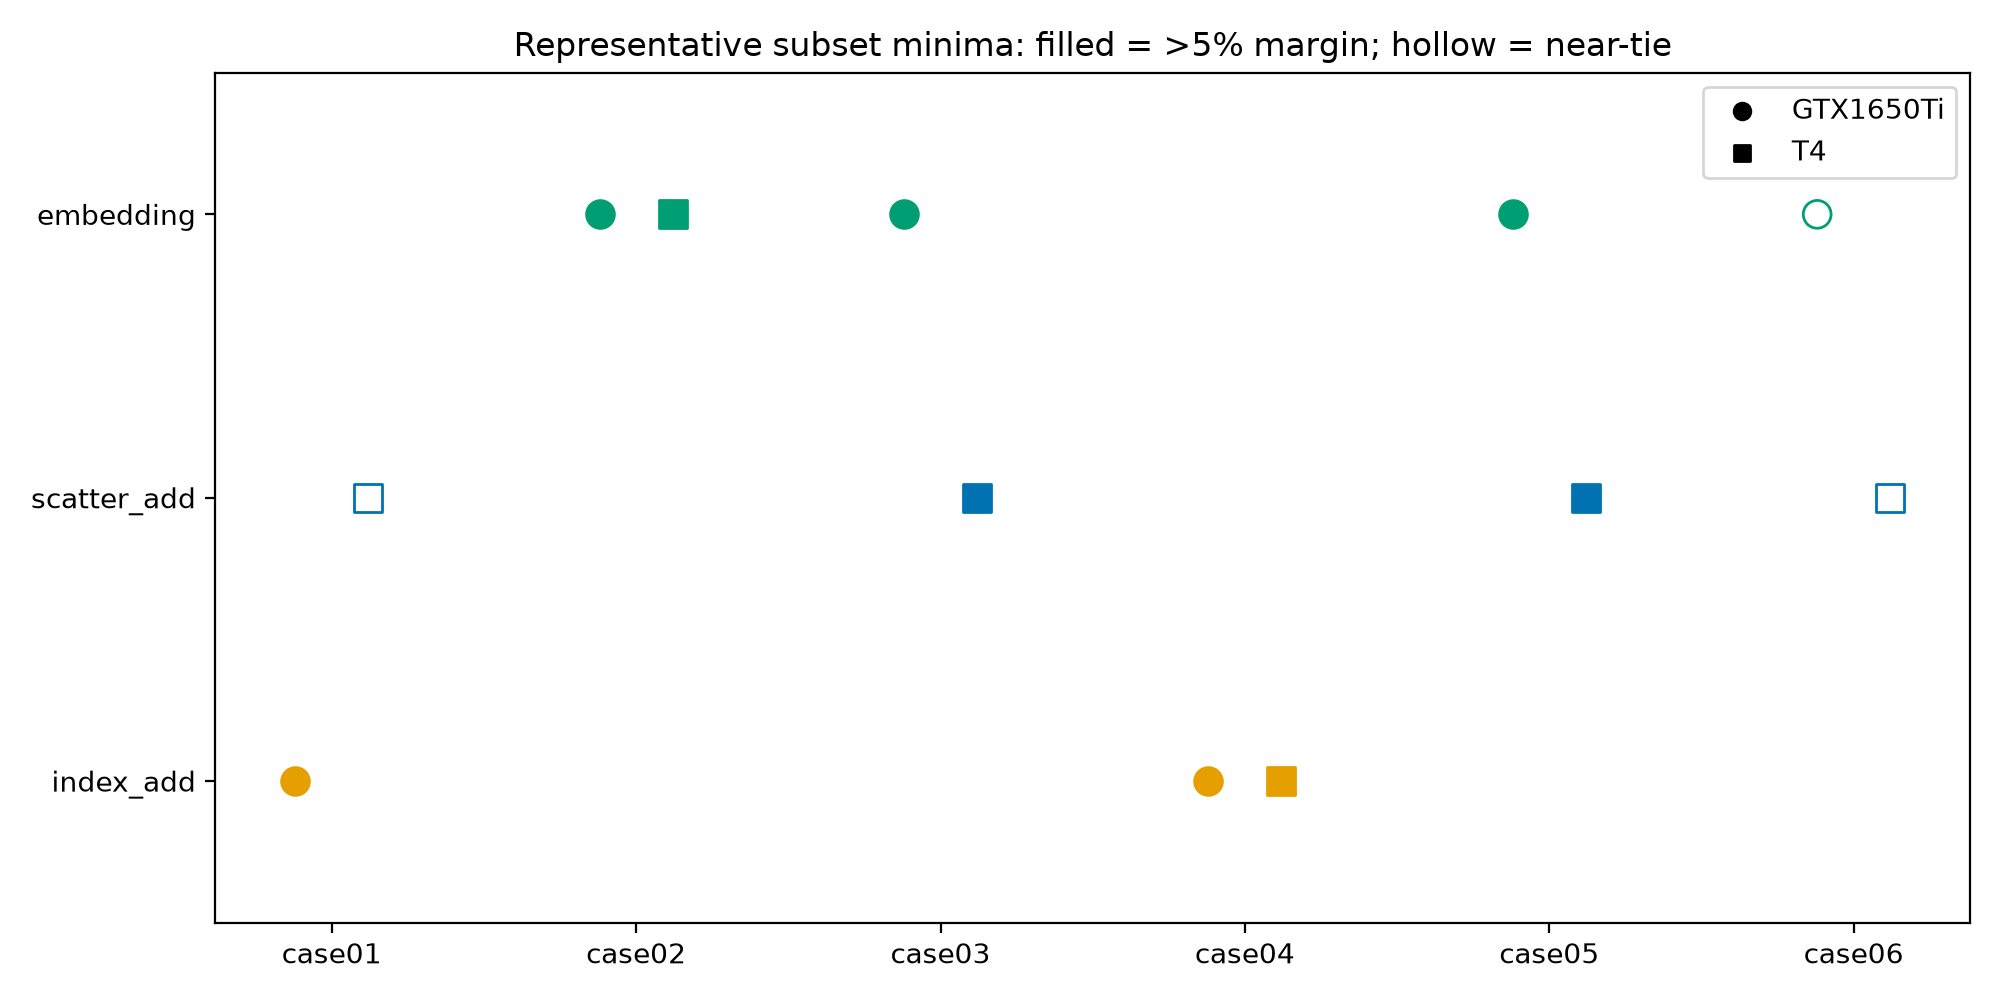
\includegraphics[width=0.80\linewidth]{figures/phase3_case_winner_comparison.png}
% TODO: \caption{Draft: Phase 3 case winner comparison.}
% TODO: \label{fig:phase3-case-winner-comparison}
% TODO: \end{figure}

\subsection{CUDA Path Attribution}
% TODO: Use phase3_comparison_v2/phase3_claim_checks.csv.
% TODO: Use phase3_comparison_v2/phase3_kernel_category_summary.csv.
% TODO: % Source: ../sparse-gradient/phase3_comparison_v2/phase3_claim_checks.csv
\begin{table}[tbp]
\centering
\small
\caption{Draft: Phase 3 claim-check status and source cautions.}
\label{tab:phase3-claim-checks}
\begin{tabular}{lp{0.12\linewidth}p{0.30\linewidth}p{0.36\linewidth}}
\toprule
Check & Passed & Supporting numbers & Caution \\
\midrule
index\_add\_path\_dominance & True & GTX1650Ti=0.9677; T4=0.9647 & Full-event CUDA category shares required. \\
scatter\_add\_path\_dominance & True & GTX1650Ti=0.9817; T4=0.9518 & Full-event CUDA category shares required. \\
embedding\_accumulation\_present & True & GTX1650Ti=0.8271; T4=0.6697 & Full-event CUDA category shares required. \\
embedding\_sort\_scan\_present & True & GTX1650Ti=0.1217; T4=0.2342 & Full-event CUDA category shares required. \\
other\_share\_controlled & True & T4/embedding=0.03467 & Unknown kernels substantial at mean other share $\geq 0.2$. \\
phase2\_environment\_difference\_present & True & GTX1650Ti=embedding; T4=scatter\_add; T4\_repeat=scatter\_add & Expected most-frequent decisive API required in all three environments. \\
representative\_reversals\_present & True & case03, case05 & Representative subset is illustrative, not statistical. \\
\bottomrule
\end{tabular}
\end{table}

\subsection{Result-Level Discussion}
% TODO: Add result-level analysis after the results narrative is finalized.
\section{General Discussion}

\subsection{Significance for AI Training Workloads}
% TODO: Discuss significance for AI training workloads.

\subsection{Practical Implications}
% TODO: Discuss practical implications.

\subsection{Limitations}
% TODO: Describe limitations.

\subsection{Generalizability}
% TODO: Discuss generalizability.

\subsection{Future Work}
% TODO: Describe future work.
\section{Conclusion}

% TODO: Write the conclusion after finalizing the evidence and discussion.

\bibliographystyle{plainnat}
\bibliography{references}

\end{document}